\documentclass[a4paper]{article}
\usepackage[utf8]{inputenc}
\usepackage{amsmath}
\usepackage{polski}
\usepackage[polish]{babel}
\usepackage[T1]{fontenc}
\usepackage[a4paper,top=3cm,bottom=2cm,left=3cm,right=3cm,marginparwidth=1.75cm]{geometry}
\usepackage{graphicx}
\usepackage{float}
\usepackage{array}
\usepackage{longtable}
\usepackage{multirow}
\usepackage{pdflscape}
\usepackage[ruled,vlined]{algorithm2e}
\usepackage[backend=bibtex]{biblatex}
\graphicspath{{../img/}}

\newcolumntype{C}[1]{>{\centering}m{#1}} 

\title{Optymalizacja fabryki z wykorzystaniem algorytmu immunologicznego (selekcji klonalnej)}
\author{Artur Bauer \and Kamil Szostek \and Sławomir Goździewski \and Wiktor Filipiak}
\date{\today}

\usepackage[pdftex,
            pdfauthor={Artur Bauer \& Kamil Szostek \& Sławomir Goździewski \& Wiktor Filipiak},
            pdftitle={\@title},
            pdfsubject={Glebokie uczenie i inteligencja obliczeniowa},
            pdfkeywords={Automatyka i Robotyka},
            pdfproducer={Latex},
            pdfcreator={pdflatex}]{hyperref}

\bibliography{citations.bib}

\begin{document}
%--------------------------------------------------------%
%	COVER PAGE
%--------------------------------------------------------%

\begin{titlepage}
\makeatletter

  \newcommand{\HRule}{\rule{\linewidth}{0.5mm}} % Defines a new command for the horizontal lines, change thickness here

  \center % Center everything on the page


%	HEADING SECTION

  \textsc{\LARGE Akademia Górniczo-Hutnicza}\\[1.5cm] % Name of your university/college
  \textsc{\Large  Głębokie uczenie i inteligencja obliczeniowa }\\[0.5cm] % Major heading such as course name
  \textsc{\large Automatyka i Robotyka II Stopień}\\[0.5cm] % Minor heading such as course title
  \textsc{2019/2020}\\[0.5cm] % Minor heading such as course title

%	TITLE SECTION

  \vspace{1.5 cm}
  \HRule \\[0.4cm]
  { \huge \bfseries \@title} \\[0.4cm] % Title of your document
  \HRule \\[1.5cm]
 
%	AUTHOR SECTION

  {\em\Large\textbf Skład zespołu:}\\
  \vspace{.5 cm}
    Artur Bauer\\
    Kamil Szostek\\
    Sławomir Goździewski\\
    Wiktor Filipiak
  \vspace{1.5 cm}
  
  
  {\em\Large\textbf Opiekun:}\\
  \vspace{.5 cm}
  dr hab. inż. Joanna Kwiecień
  
%	DATE SECTION

  \vspace{1.5 cm}
  {\large Złożono: \@date}\\[3cm] % Date, change the \today to a set date if you want to be precise


\vfill % Fill the rest of the page with whitespace

\end{titlepage}

%-----------------------------------------------------------------

\newpage

\tableofcontents

\newpage
\section{Wstęp}
\subsection{Model fabryki}\label{factory}

\begin{figure}[ht]
\centering
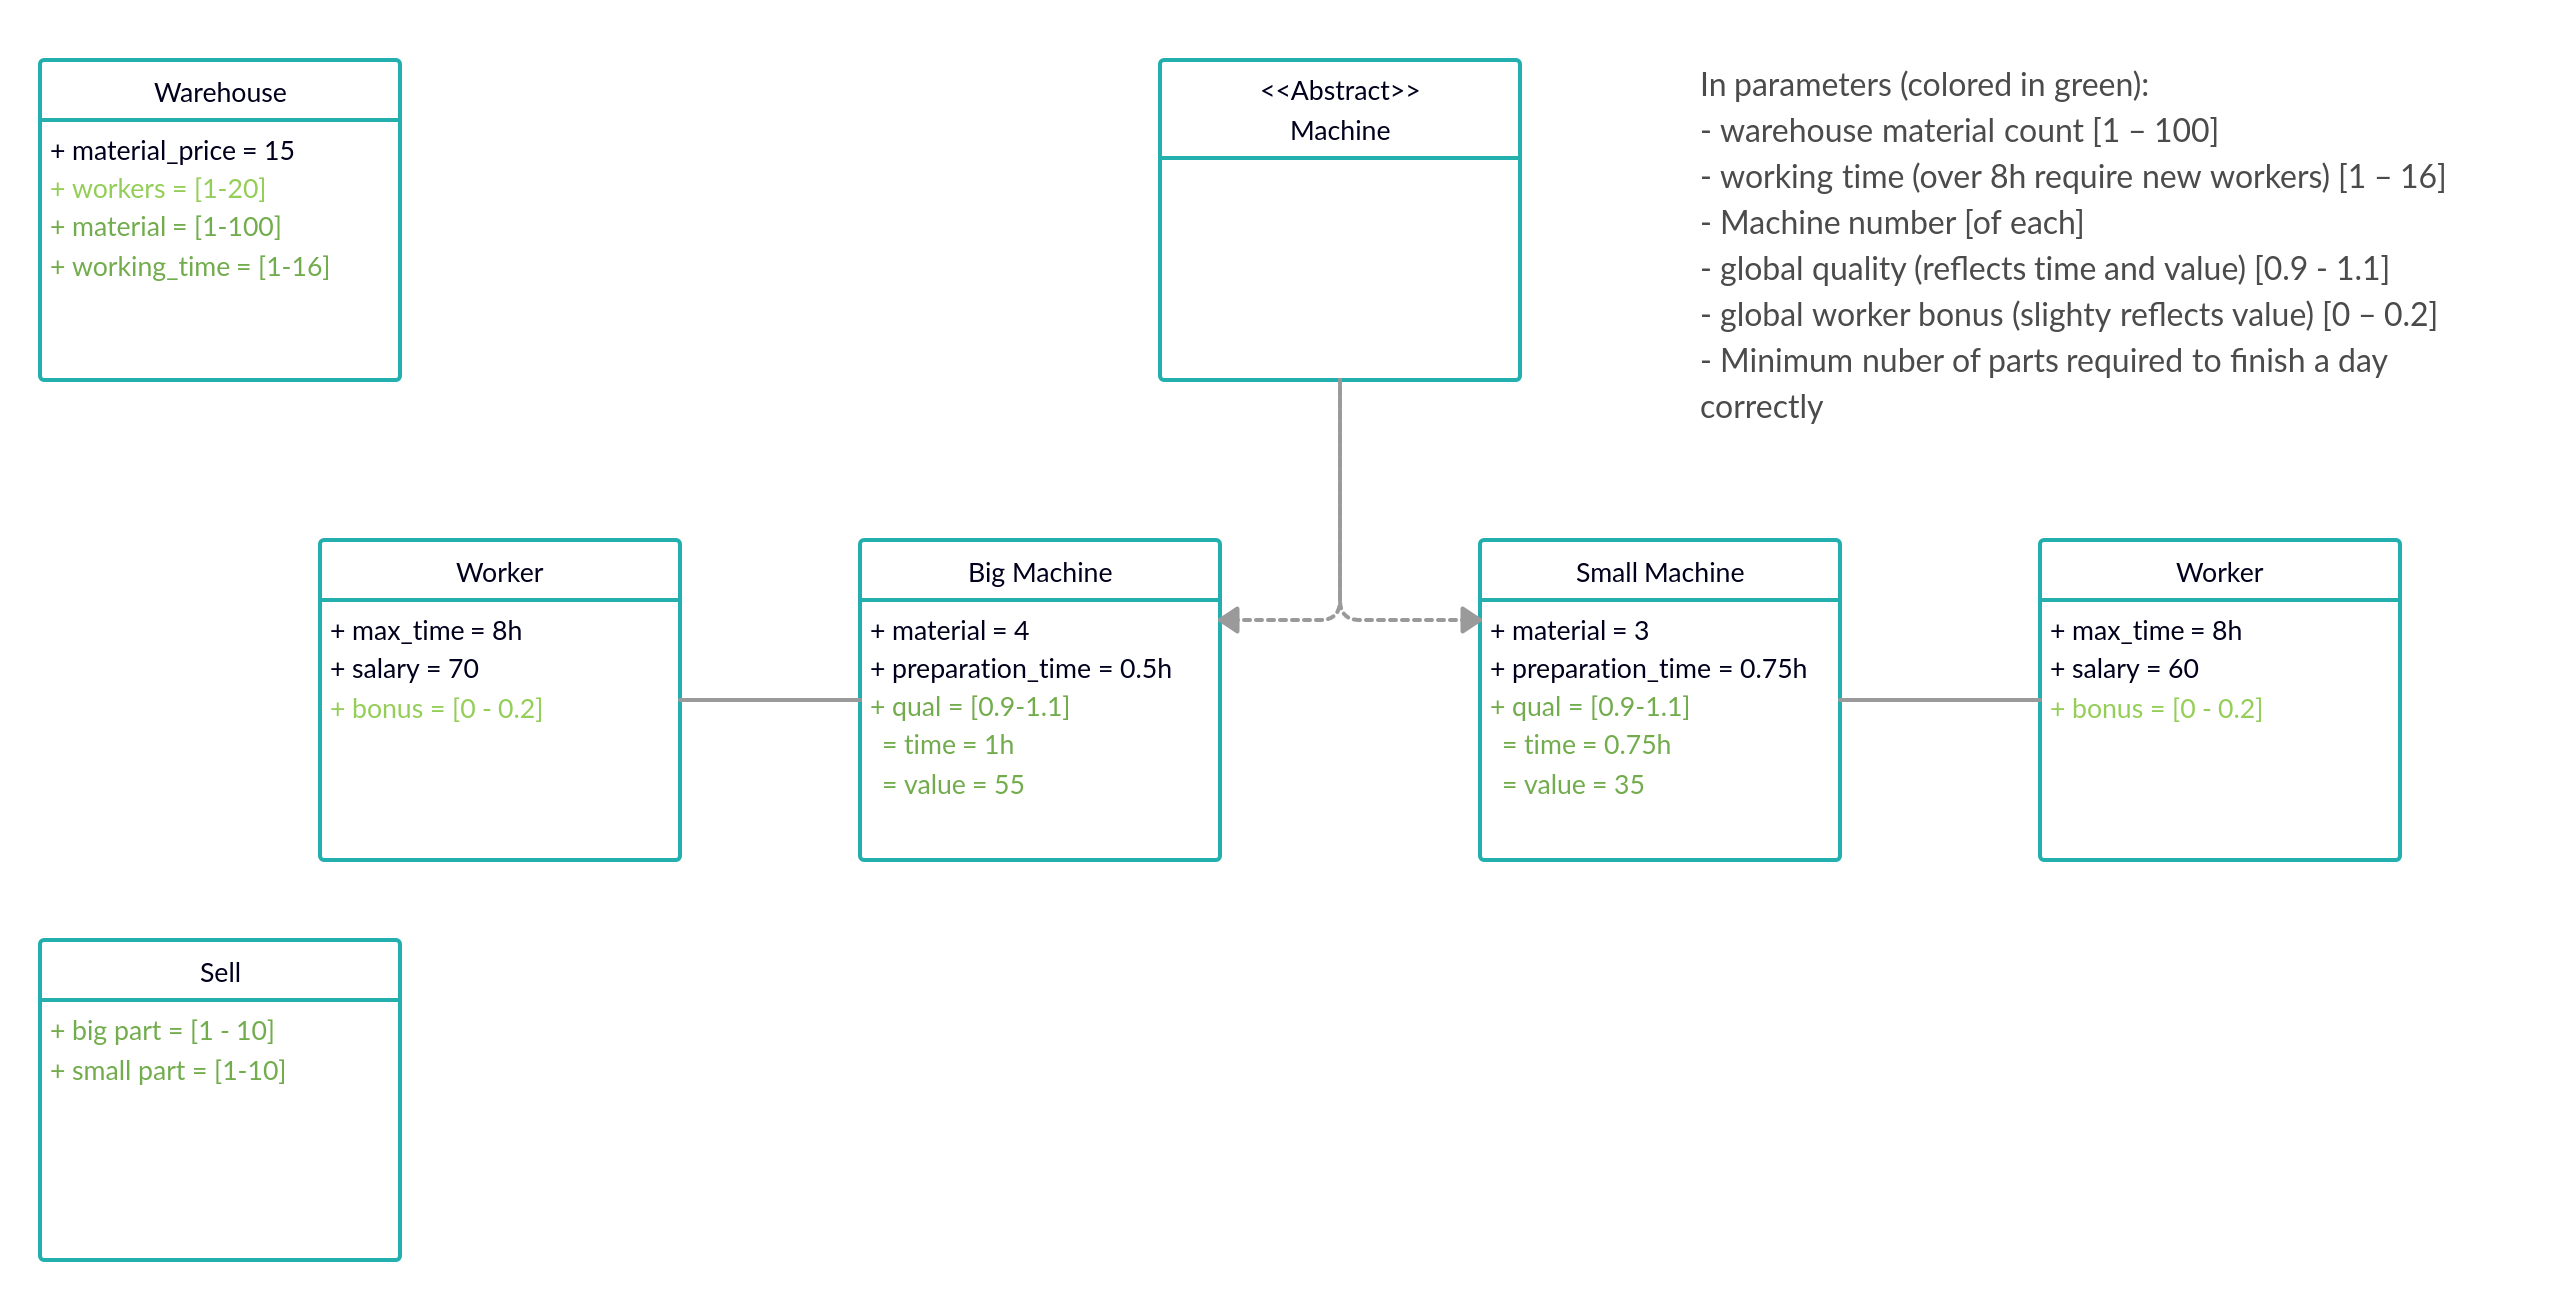
\includegraphics[width=.7\textwidth]{Factory_scheme.png}
\caption{Factory scheme}
\end{figure}

\subsubsection{Funkcja celu fabryki:}\label{factory-main-goal-function}

$$Income = \sum^{n_p}_{i=1}(p_i*(v_i-m_i*m_p)) - (1+b_i)*\sum^{n_w}_{i = 1}(w_i*s_i *t_{wi}) - m_r*m_p - punish$$

Gdzie:
\begin{itemize}
    \item $n_p$ -- ilość rodzajów części
    \item $p_i (n_m)$ -- ilość wyprodukowanych części i-tego typu
    \item $v_i(v_{bi}, t_{wi},t_{bi},w_q)$ -- wartość części i-tego typu
    \item $m_i$ -- liczba surowca potrzebna do wytworzenia elementu i-tego typu
    \item $m_p$ -- cena surowca
    \item $n_w$ -- liczba rodzajów pracowników
    \item $w_i$ -- liczba pracowników i-tego rodzaju
    \item $s_i$ -- wypłata pracownika i-tego rodzaju
    \item $b$ -- premia pracownicza
    \item $m_r(p_i,n_m)$ -- pozostały materiał
    \item $p_{i_{min}}$ -- minimalna ilość elementów do wytworzenia i uniknięcia kary
    \item $p_{i_{max}}$ -- maksymalna ilość wytworzonych elementów
    \item $n_m$ -- liczba surowca na początek dnia
\end{itemize}
\subsubsection{Kara}
$punish = p_{un}*\sum^{n_p}_{i=1}(p_{num_i})*v_i$

$p_{num_i}= \left\{\begin{matrix} 0  \;\quad\quad\quad\quad  \textrm{if} \quad  p_{i_{min}}-p_i \leq  0    \\ p_{i_{min}}-p_i  \quad  \textrm{if} \quad  p_{i_{min}}-p_i >  0  \end{matrix}\right.$

Gdzie: 
\begin{itemize}
    \item $p_{un}$ -- współczynnik kary
    \item $p_{num_i}(p_{i_{min}}, p_i)$ -- liczba elementów i-tego typu dla których naliczana jest kara
\end{itemize}
\subsubsection{Liczba pracowników}

Liczba pracowników i-tego typu jest równa ilości maszyn i-tego typu:

$n_p = n_w$

\subsubsection{Maksymalna ilość elementów}\label{max-number-of-items}

Niezbędna ilość elementów i-tego typu:

$\sum^{n_p}_{i=1} p_{i_{max}} * m_i< n_m$

\subsubsection{Rzeczywisty czas pracy maszyny na 1 produkt}\label{real-working-time-of-the-i-type-machineemployee-for-one-product} 
$t_{wi} = t_{pi} + p_i * t_{bi}$

\subsection{Parametry modelu}\label{model-assumption}

\begin{longtable}[c]{lll}
Parametr & oznaczenie & wartość\\ \hline
Ilość surowców & $n_m$ & [$x$ - 100 $x$]\\
Koszt surowca & $m_p$ & 4\\
Czas pracy & $t_f$ & [1 - 16]\\
Minimalna ilość dużych części & $p_{0_{min}}$ & [0 - 10]\\
Minimalna ilość małych części & $p_{1_{min}}$ & [0 -10]\\
Wypłata operatora dużej maszyny & $s_0$ & 19\\
Wymagana ilość materiału na duży element & $m_0$ & 6\\
Czas przygotowania dużej maszyny & $t_{p0}$ & 1h 45 min\\
Wartość dużego elementu & $v_{b0}$ & 70\\
Podstawowy czas pracy na duży element & $t_{b0}$ & 1h\\
Liczba dużych maszyn & $c_0$ & [0 - 30]\\
Wypłata operatora małej maszyny & $s_1$ & 17\\
Ilość surowca na mały element & $m_1$ & 4\\
Czas przygotowania małej maszyny & $t_{p1}$ & 1h 25 min\\
Wartość małego elementu & $v_{b1}$ & 50\\
Czas wytworzenia małego elementu & $t_{b1}$ & 1h 25 min\\
Ilość małych maszyn & $c_1$ & [0 - 30]\\
Maksymalny czas pracy pracownika & $t_w$ & 8h\\
Bonus pracowniczy & b & [0.0 - 0.5]\\
Współczynnik kary & $p_{un}$ & [0 - 1]
\end{longtable}

Gdzie:
\begin{itemize}
    \item $x$ -- ilość wymaganych elementów * koszt części 
    \item Parametry wejściowe podane są w kwadratowych nawiasach
    \item Pracownik jest zatrudniony na pełen etat (8h płacone z góry)
    \item Pierwsza i druga zmiana są identyczne w ilość i rodzaj maszyn i pracowników
    \item Rezerwujemy surowce na wymagane elementy
    \item Wszystkie elementy ponad wymaganą liczbę są ekstra dochodem
\end{itemize}


\section{Badany problem}
\subsection{Przegląd literatury}
Artykuł dotyczy algorytmu selekcji klonalnej stosowanej do optymalizacji w elektromagnetyce. Autorzy prezentują ich własną koncepcję kodowanego algorytmu selekcji klonalnej, który może zostać użyty w elektromagnetycznej optymalizacji projektu, a także sposób działania algorytmu dla problemu "The TEAM Workshop problem 22”.\cite{1430953}.

Artykuł przedstawia zastosowanie sztucznego systemu immunologicznego w aplikacji przemysłowej. Na postawie parametrów obróbki (siła, moment, itp.) oraz zakłócenia (wibracje, itp.) autorzy wykrywają uszkodzenie narzędzia. Wykorzystywany jest algorytm sztucznego systemu immunologicznego wykorzystuje do działania algorytm selekcji negatywnej \cite{dasgupta1999artificial}.

Artykuł przedstawia użycie algorytmów sztucznych systemów immunologicznych w przemyśle. Porównuje on algorytmy sztucznej inteligencji z algorytmem klonowania do algorytmu z mechanizmem uczenia społecznego. Zmieniając wzmocnienie, czas zdwojenia oraz czas wyprzedzenia dobierają one nastawy regulatora PID \cite{wang_artificial_2017}.

Artykuł dotyczy algorytmu selekcji klonalnej opartego na algorytmach memetycznych stosowanego do problemów planowania zadań. Autorzy skupili się na poprawie eksploracji i eksploatacji przy użyciu algorytmu selekcji klonalnej. W artykule przedstawiono użycie selekcji klonalnej do skonstruowania ewolucyjnego mechanizmu wyszukiwania wykorzystywanego do eksploracji.\cite{yang2008clonal}.

Artykuł przedstawia użycie Algorytmu Selekcji Klonalnej w zastosowaniach inżynierskich. Opisane w nim jest działanie algorytmu od strony teoretycznej, a także działanie zaimplementowanego przez autorów algorytmu przy rozwiązywaniu trzech różnych problemów: binarnego rozpoznawania znaków, wielomodalnej optymalizacji funkcji -
$f(x, y) = x.\sin{4 \pi x} - y.\sin{4 \pi y + \pi} + 1$
i problemu komiwojażera dla 30 miast \cite{de_castro}.


Artykuł przedstawia użycie Algorytmu Selekcji Klonalnej do optymalizacji ułożenia terenu budowy. Zaprezentowany algorytm minimalizuje koszty produkcji i dystans przebyty pomiędzy n obiektami zaprezentowanymi za pomocą macierzy permutacji o wymiarach n x n \cite{WANG2016267}.


Artykuł przedstawia działanie sztucznego systemu immunologicznego (AIS) w przypadku rozwiązania pojemnościowego problemu marszrutyzacji. Celem było znalezienie odpowiedniego zestawienia parametrów algorytmu selekcji klonalnej w celu rozwiązania problemu poprzez podejście eksperymentalne. W artykule oprócz działania AIS, opisano także działanie innych metod rozwiązujących dwadzieścia instancji problemu i przedstawiono wyniki pod względem jakości rozwiązań oraz wykorzystanego czasu obliczeniowego \cite{thapatsuwan}.


Artykuł dotyczy zastosowania algorytmu selekcji klonalnej w celu określenia optymalnych punktów pracy w niskonapięciowych, hybrydowych mikrosieciach AC/DC. Celem było zminimalizowanie strat mocy czynnej, kosztów eksploatacji oraz optymalizacja napięcia węzłowego \cite{rokicki}.


\section{Diagram UML fabryki}
\begin{figure}[ht]
\centering
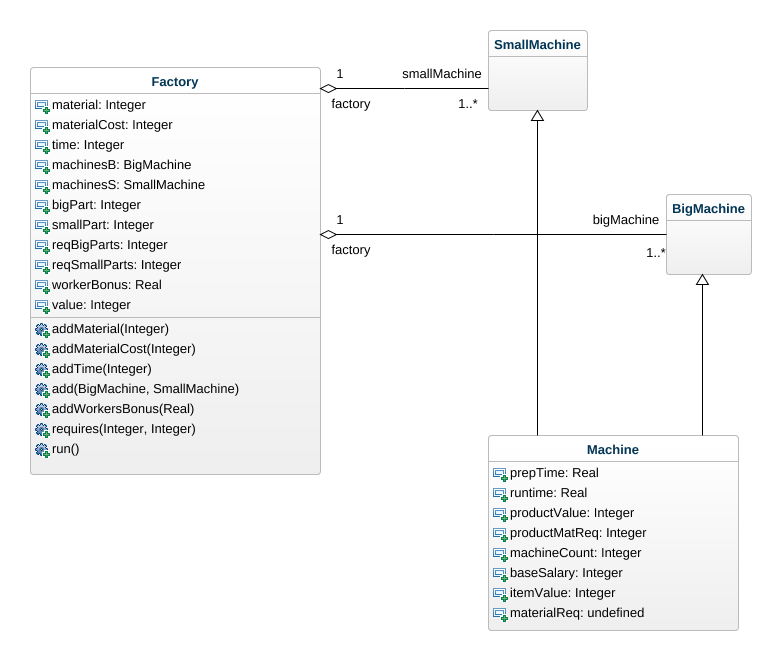
\includegraphics[width=.7\textwidth]{UML_Model.png}
\caption{Diagram UML}
\end{figure}

\section{Algorytm}
Do optymalizacji fabryki zdecydowano się na wybór algorytmu immunologicznego z wykorzystaniem selekcji klonalnej.

Algorytm ten wykorzystuje populację przeciwciał, które są odpowiednikami punktów w wielowymiarowej przestrzeni rozwiązań.
Najpierw w sposób losowy tworzona jest populacja przeciwciał które zostają zoptymalizowane.
Proces optymalizacji polega na poszukiwaniu przeciwciał maksymalizujących (lub minimalizujących) funkcję celu.
Z populacji wybierane są najlepsze przeciwciała które następnie są klonowane.
Spośród wybranych przeciwciała o najlepszym dopasowaniu (wyniku) są klonowane wielokrotnie, natomiast ilość klonów przeciwciał o niższym dopasowaniu jest niższa.
Następnie klony są poddawane mutacjom których wielkość jest odwrotnie proporcjonalna do ich jakości. Klony o największym dopasowaniu mutowane są delikatnie, natomiast klony o mniejszym dopasowaniu podlegają większym mutacjom. Następnie każde oryginalne przeciwciało jest z pewnym prawdopodobieństwem zastępowane klonem (o ile ten jest lepszej jakości). Proces jest powtarzany do momentu w którym w kolejnych populacjach nie będą dostrzegalne zmiany lub osiągnięta zostanie odpowiednia liczba iteracji.
Pseudokod algorytmu został przedstawiony w algorytmie~\ref{alg:clolang}.

\subsection{Pseudokod}
\begin{algorithm}[H]
\label{alg:clolang}
\SetAlgoLined
\caption{Pseudokod algorytmu immunologicznego z wykorzystaniem selekcji klonalnej}
\KwData{population\_size, selection\_rate, clone\_rate}
\KwResult{bestSolution}
\Begin{
    population $ \longleftarrow $ generate\_population(population\_size)\;
    \While{stop criteria is not met}{
        selected $ \longleftarrow $ select(population, math.ceil(selection\_rate * population\_size))\;
        clones $ \longleftarrow $ clone(selected, clone\_rate)\;
        matured $ \longleftarrow $ hypermutate(clones)\;
        population $ \longleftarrow $ replace(population, matured)\;
    }

    bestSolution $ \longleftarrow $\ selectBest(population)\;
}
\end{algorithm}

\section{Testy}

Wykonano szereg testów dla różnych parametrów algorytmu immunologicznego. 
Jako podstawowe parametry przyjęto: rozmiar populacji = 100, ilość iteracji = 200, współczynnik wybranych komórek =20\% współczynnik klonowania = 50\% i watchdog = 50.
Najlepszym wynikiem osiągniętym było $1612.46$ w 183 iteracji. Wykres uczenia został przedstawiony na rys.~\ref{fig:default_run}.

\begin{table}[h]
    \centering
    \caption{Wpływ parametrów na proces optymalizacji}
    \begin{tabular}{m{30mm} m{10mm} l m{30mm} m{30mm}}
        \multicolumn{5}{c}{\textbf{Wpływ liczby populacji}} \\ \hline
        Liczba populacji & Rysunek & Najlepsza wartość & Iteracja z \newline najlepszą wartością & Najlepsze \newline rozwiązanie \\
        10  & rys.~\ref{fig:population_10} & $-795.31$ & 74 & \multirow{4}{*}{$1825.85$} \\
        40  & rys.~\ref{fig:population_40} & $ 971.91$ & 20 &  \\
        200 & rys.~\ref{fig:population_200}& $1739.31$ & 55 &  \\
        500 & rys.~\ref{fig:population_500}& $1825.85$ & 94 &  \\
        
        \multicolumn{5}{c}{\textbf{Wpływ liczby iteracji}} \\ \hline
        Liczba iteracji & Rysunek & Najlepsza wartość & Iteracja z \newline najlepszą wartością & Najlepsze\newline rozwiązanie \\
        10  & rys.~\ref{fig:iteration_10} & $-167.0$ & 10 & \multirow{4}{*}{$1680.4$} \\
        40  & rys.~\ref{fig:iteration_40} & $1216.45$ & 37 &  \\
        100 & rys.~\ref{fig:iteration_100}& $ 844.96$ & 73 &  \\
        500 & rys.~\ref{fig:iteration_500}& $1680.4$ & 91 &  \\
        
        \multicolumn{5}{c}{\textbf{Wpływ współczynnika klonowania}} \\ \hline
        Współczynnik \newline klonowania & Rysunek & Najlepsza wartość & Iteracja z \newline najlepszą wartością & Najlepsze \newline rozwiązanie \\
        0.25 & rys.~\ref{fig:clone_025} & $ 819.73$ & 26 & \multirow{4}{*}{$1615.86$} \\
        0.40 & rys.~\ref{fig:clone_040} & $1547.17$ & 113 &  \\
        0.60 & rys.~\ref{fig:clone_060} & $1615.86$ & 172 &  \\
        0.80 & rys.~\ref{fig:clone_080} & $ 865.72$ & 74 &  \\
        
        \multicolumn{5}{c}{\textbf{Wpływ watchdog'a}} \\ \hline
        Watchdog & Rysunek & Najlepsza wartość & Iteracja z \newline najlepszą wartością & Najlepsze\newline rozwiązanie \\
        5  & rys.~\ref{fig:watchdog_05} & $-101.07$ & 19 & \multirow{4}{*}{$1767.93$} \\
        40 & rys.~\ref{fig:watchdog_40} & $ 843.33$ & 20 &  \\
        60 & rys.~\ref{fig:watchdog_60} & $ 948.33$ & 59 &  \\
        80 & rys.~\ref{fig:watchdog_80} & $1767.93$ & 151 &  \\
        
        \multicolumn{5}{c}{\textbf{Wpływ współczynnika wybranych komórek}} \\ \hline
        Współczynnik \newline wybranych \newline komórek & Rysunek & Najlepsza wartość & Iteracja z \newline najlepszą wartością & Najlepsze\newline rozwiązanie \\
        0.05 & rys.~\ref{fig:selection_05} & $1178.58$ & 75 & \multirow{4}{*}{$1255.00$} \\
        0.10 & rys.~\ref{fig:selection_10} & $ 558.54$ & 24 &  \\
        0.40 & rys.~\ref{fig:selection_40} & $1255.00$ & 57 &  \\
        0.50 & rys.~\ref{fig:selection_50} & $ 807.50$ & 46 &  \\
    \end{tabular}
    \label{tab:testy}
\end{table}

\subsection{Wykresy}

\begin{figure}[H]
    \centering
    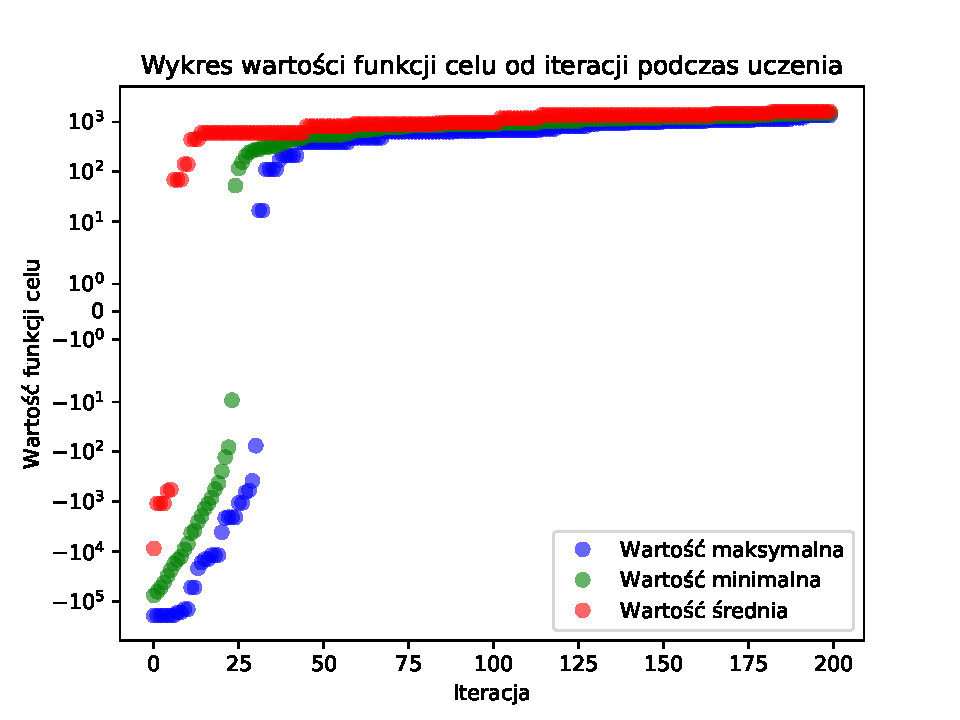
\includegraphics[width=0.7\textwidth]{plots/Default_run.pdf}
    \caption{Przebieg na podstawowych parametrach}
    \label{fig:default_run}
\end{figure}

\subsubsection{Wpływ populacji}
\begin{figure}[H]
    \centering
    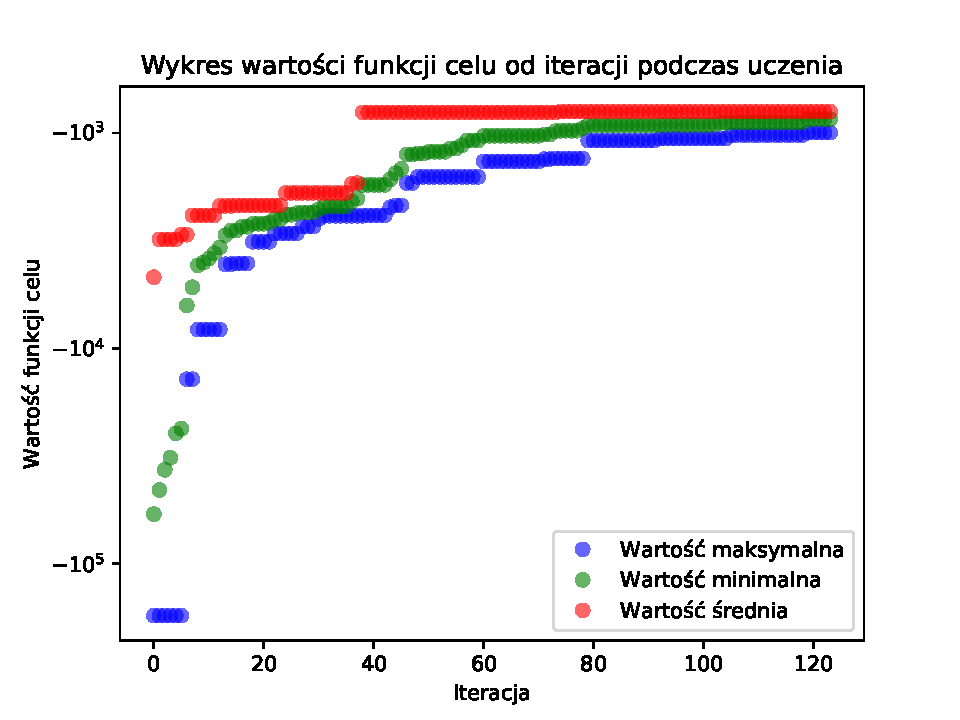
\includegraphics[width=0.7\textwidth]{plots/population_10.pdf}
    \caption{Populacja = 10}
    \label{fig:population_10}
\end{figure}

\begin{figure}[H]
    \centering
    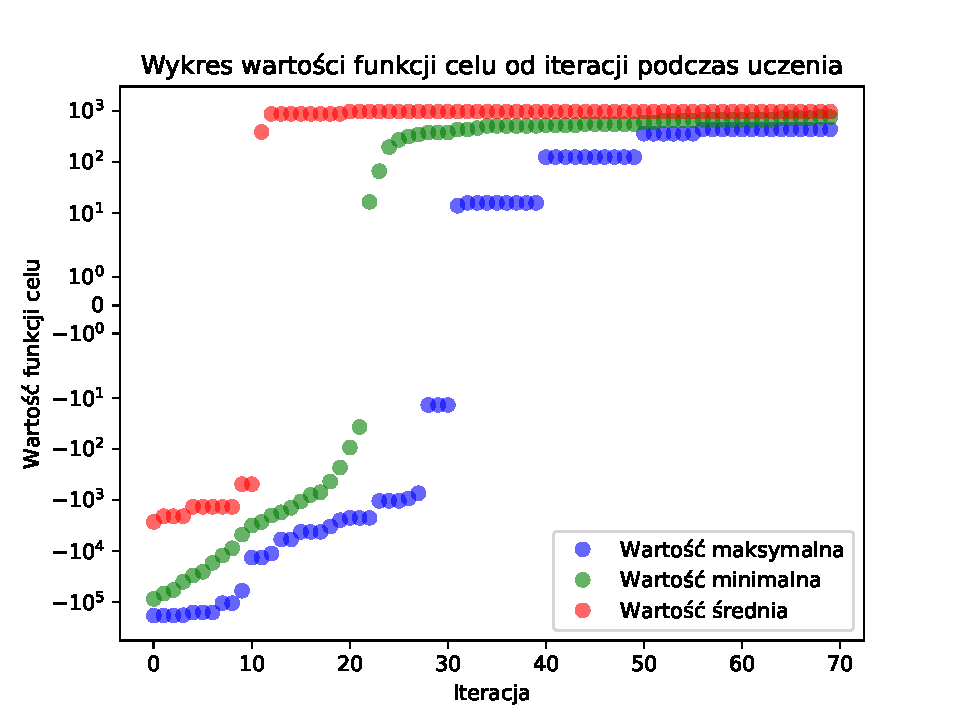
\includegraphics[width=0.7\textwidth]{plots/population_40.pdf}
    \caption{Populacja = 40}
    \label{fig:population_40}
\end{figure}

\begin{figure}[H]
    \centering
    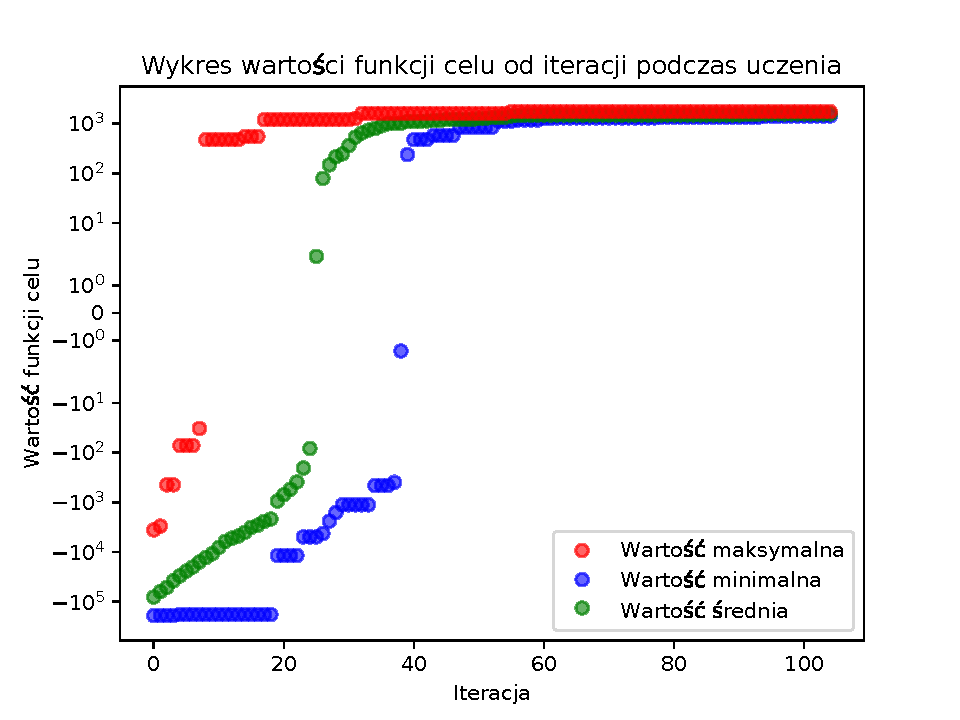
\includegraphics[width=0.7\textwidth]{plots/population_200.pdf}
    \caption{Populacja = 200}
    \label{fig:population_200}
\end{figure}

\begin{figure}[H]
    \centering
    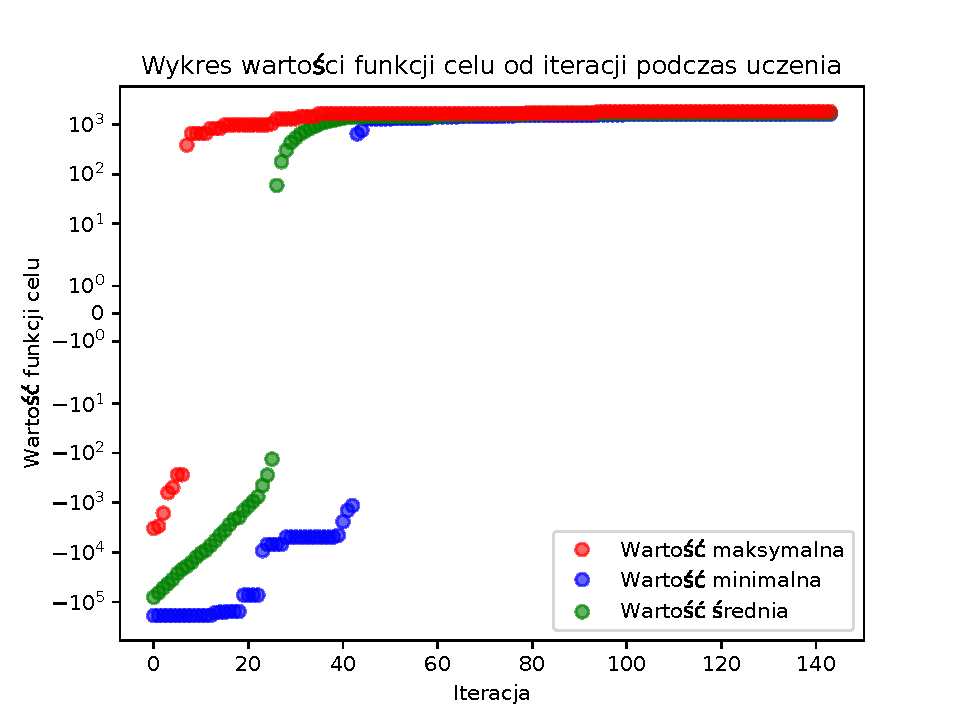
\includegraphics[width=0.7\textwidth]{plots/population_500.pdf}
    \caption{Populacja = 500}
    \label{fig:population_500}
\end{figure}


\subsubsection{Wpływ iteracji}

\begin{figure}[H]
    \centering
    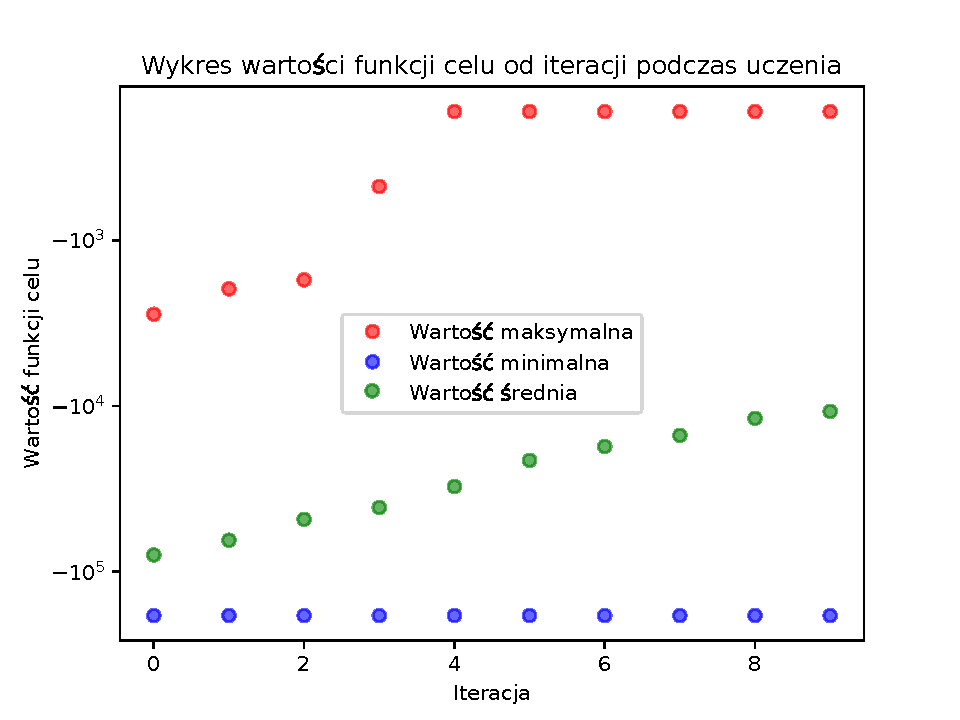
\includegraphics[width=0.7\textwidth]{plots/iteration_10.pdf}
    \caption{Iteracje = 10}
    \label{fig:iteration_10}
\end{figure}

\begin{figure}[H]
    \centering
    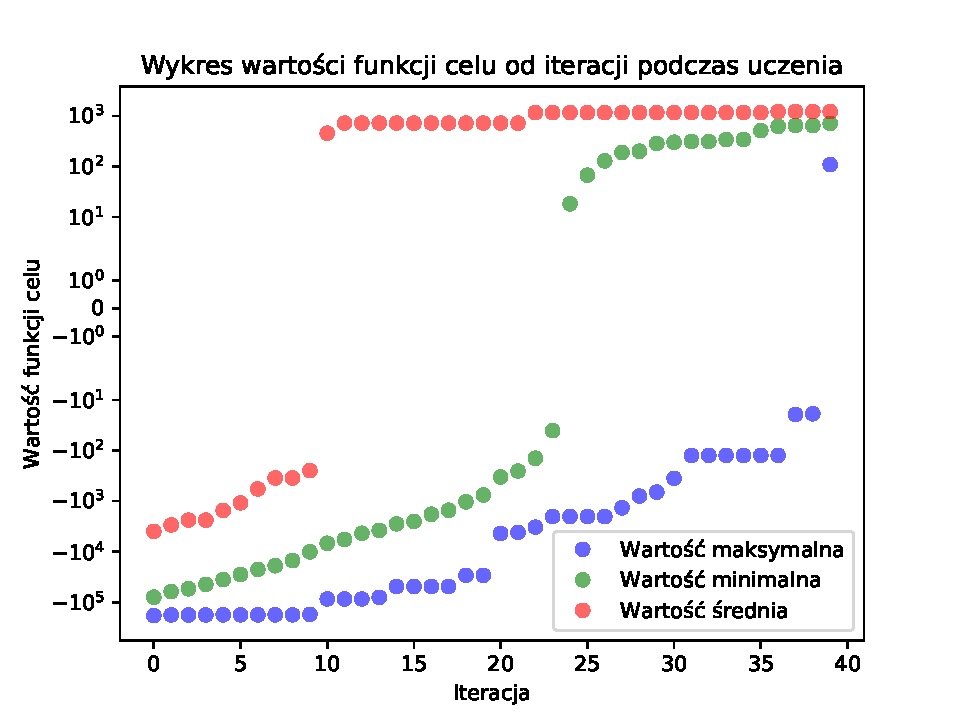
\includegraphics[width=0.7\textwidth]{plots/iteration_40.pdf}
    \caption{Iteracje = 40}
    \label{fig:iteration_40}
\end{figure}

\begin{figure}[H]
    \centering
    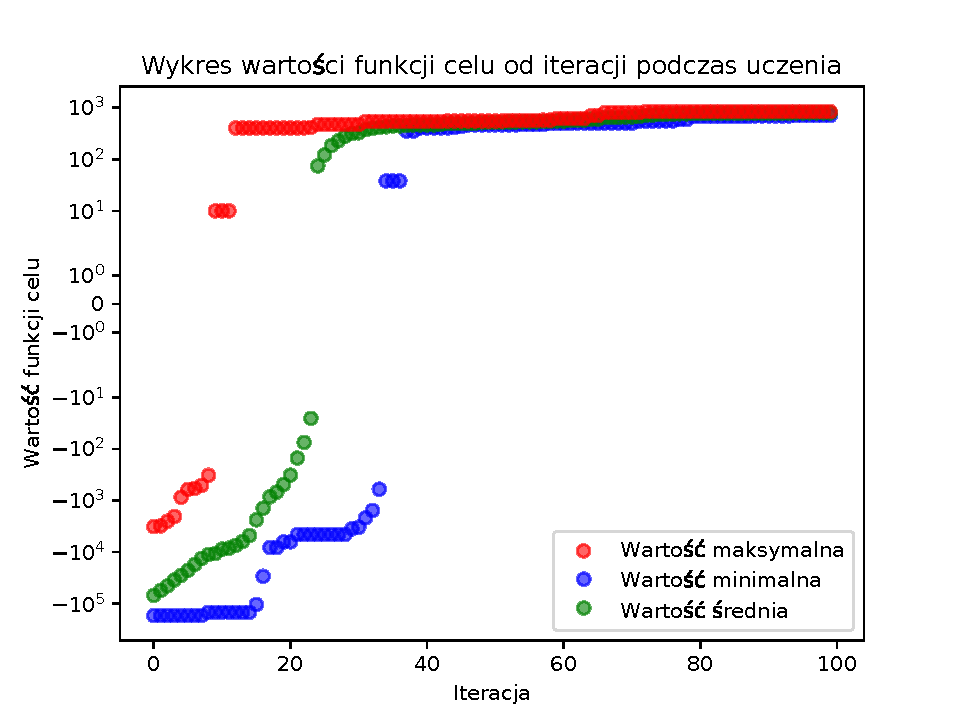
\includegraphics[width=0.7\textwidth]{plots/iteration_100.pdf}
    \caption{Iteracje = 100}
    \label{fig:iteration_100}
\end{figure}

\begin{figure}[H]
    \centering
    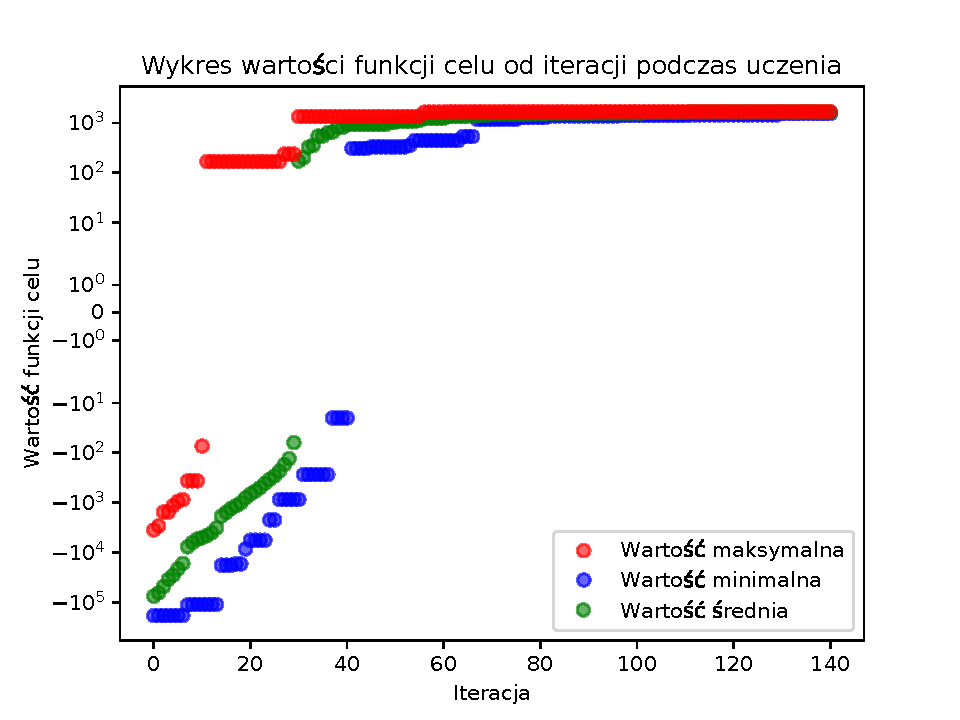
\includegraphics[width=0.7\textwidth]{plots/iteration_500.pdf}
    \caption{Iteracje = 500}
    \label{fig:iteration_500}
\end{figure}


\subsubsection{Wpływ współczynnika klonowania}

\begin{figure}[H]
    \centering
    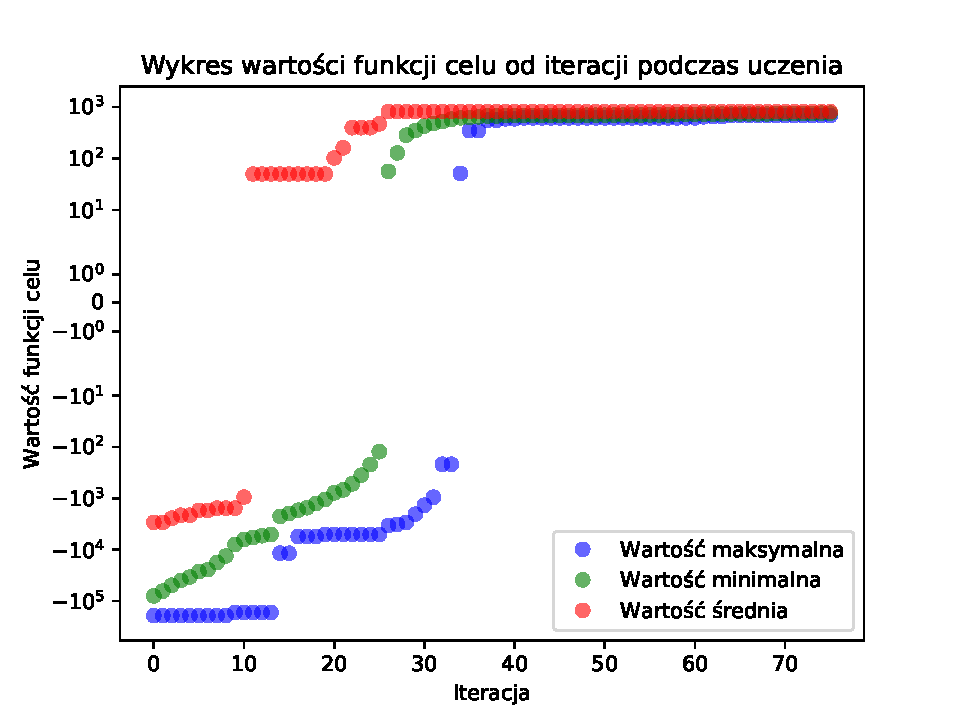
\includegraphics[width=0.7\textwidth]{plots/clone_025.pdf}
    \caption{Współczynnik klonowania = 25\%}
    \label{fig:clone_025}
\end{figure}

\begin{figure}[H]
    \centering
    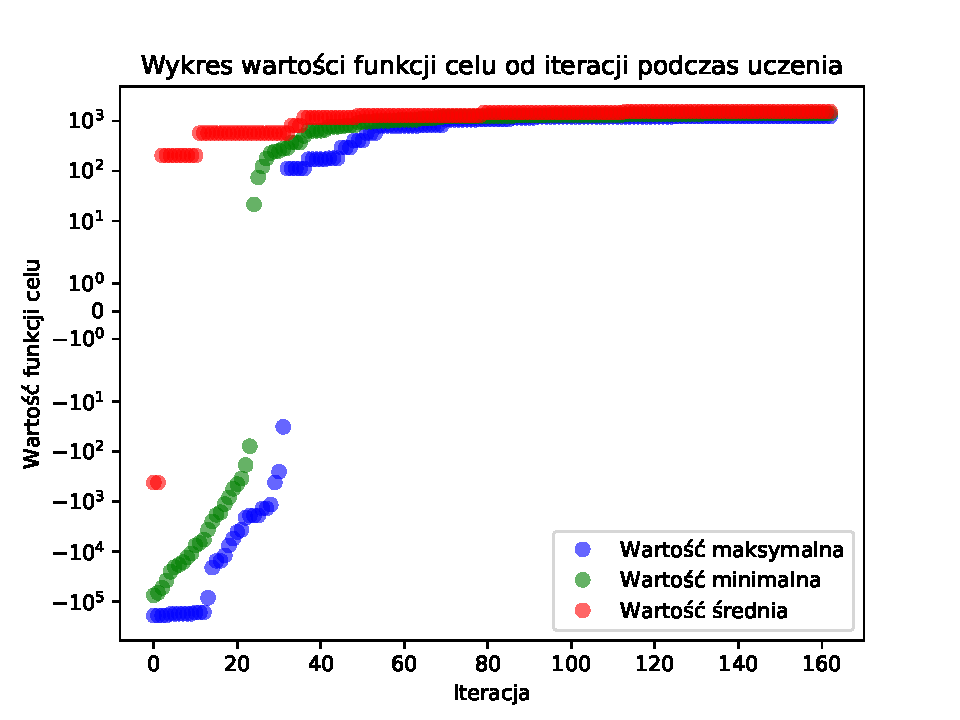
\includegraphics[width=0.7\textwidth]{plots/clone_040.pdf}
    \caption{Współczynnik klonowania = 40\%}
    \label{fig:clone_040}
\end{figure}

\begin{figure}[H]
    \centering
    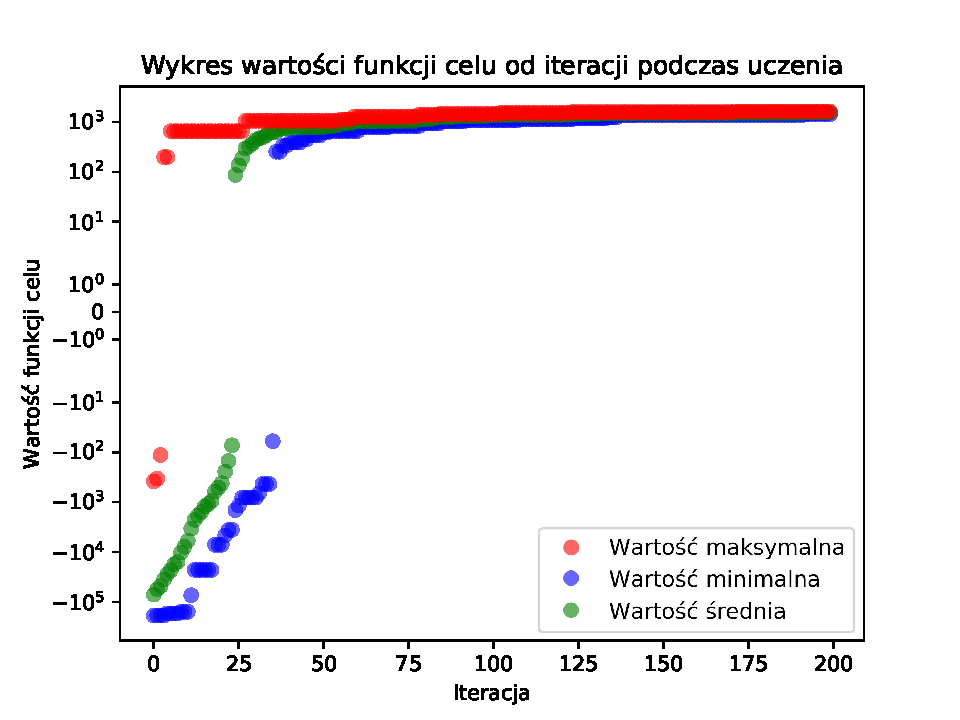
\includegraphics[width=0.7\textwidth]{plots/clone_060.pdf}
    \caption{Współczynnik klonowania = 60\%}
    \label{fig:clone_060}
\end{figure}

\begin{figure}[H]
    \centering
    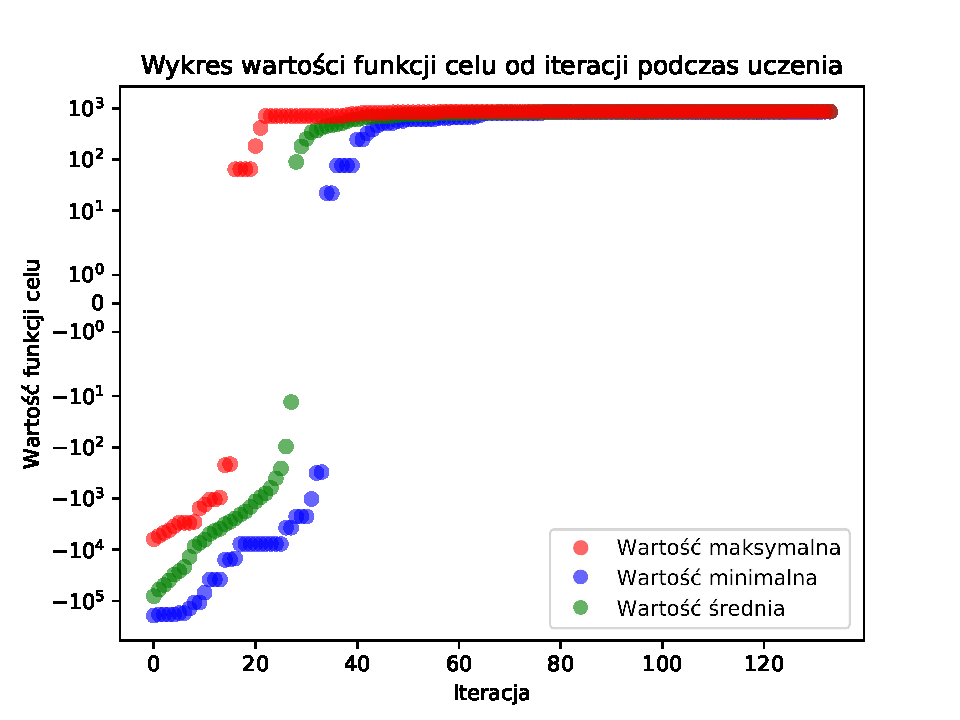
\includegraphics[width=0.7\textwidth]{plots/clone_080.pdf}
    \caption{Współczynnik klonowania = 80\%}
    \label{fig:clone_080}
\end{figure}

\subsubsection{Wpływ watchdog'a}
\begin{figure}[H]
    \centering
    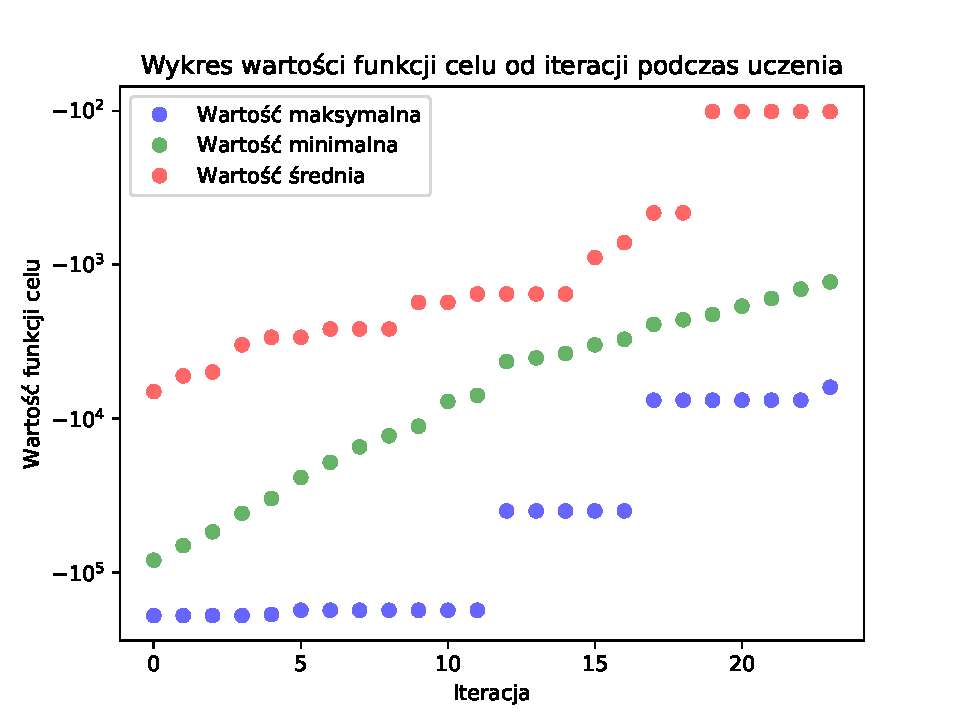
\includegraphics[width=0.7\textwidth]{plots/watchdog_05.pdf}
    \caption{Watchdog = 5}
    \label{fig:watchdog_05}
\end{figure}

\begin{figure}[H]
    \centering
    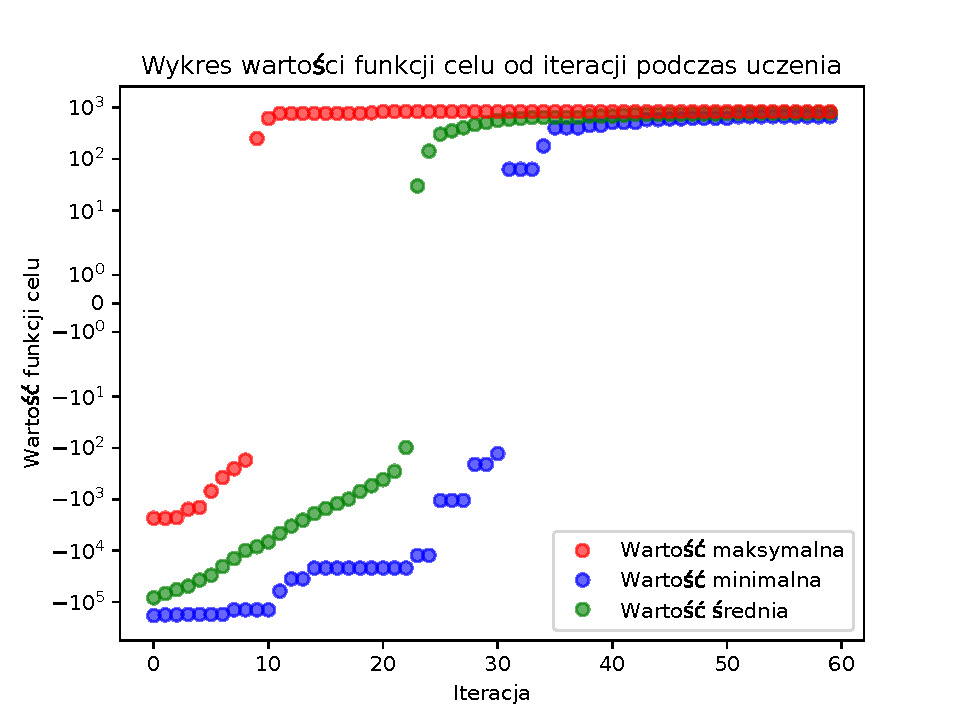
\includegraphics[width=0.7\textwidth]{plots/watchdog_40.pdf}
    \caption{Watchdog = 40}
    \label{fig:watchdog_40}
\end{figure}

\begin{figure}[H]
    \centering
    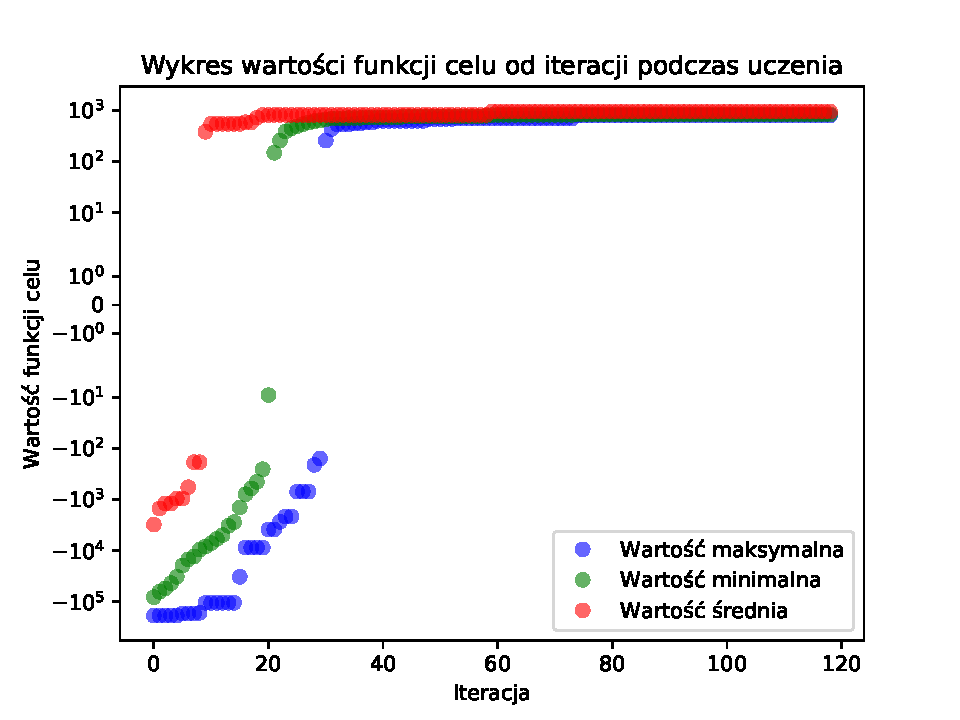
\includegraphics[width=0.7\textwidth]{plots/watchdog_60.pdf}
    \caption{Watchdog = 60}
    \label{fig:watchdog_60}
\end{figure}

\begin{figure}[H]
    \centering
    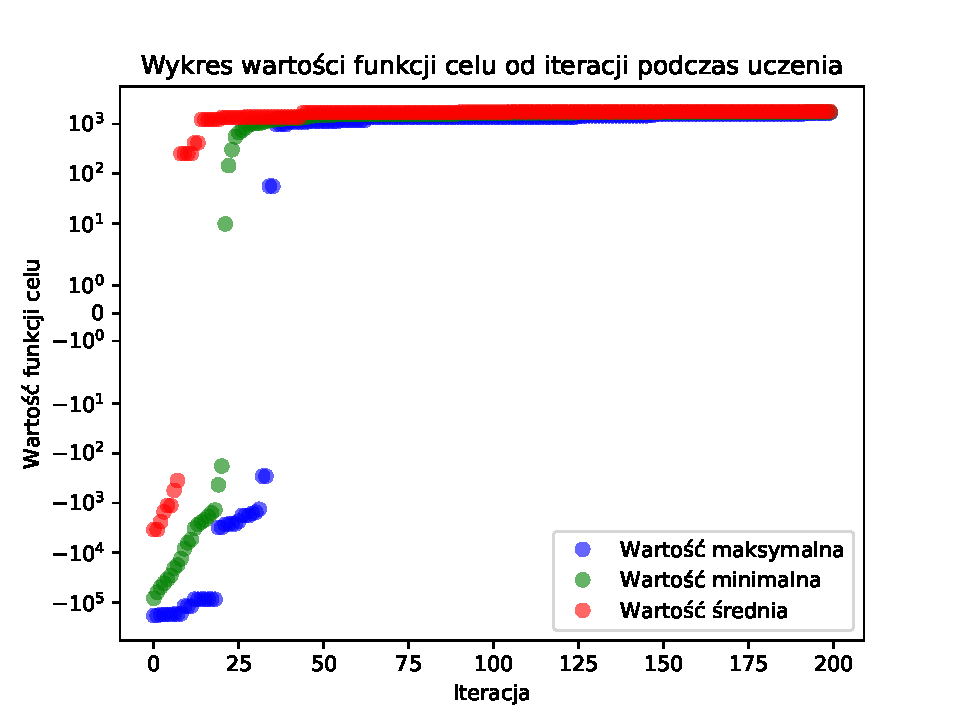
\includegraphics[width=0.7\textwidth]{plots/watchdog_80.pdf}
    \caption{Watchdog = 80}
    \label{fig:watchdog_80}
\end{figure}


\subsubsection{Wpływ współczynnika wybieranych komórek}
\begin{figure}[H]
    \centering
    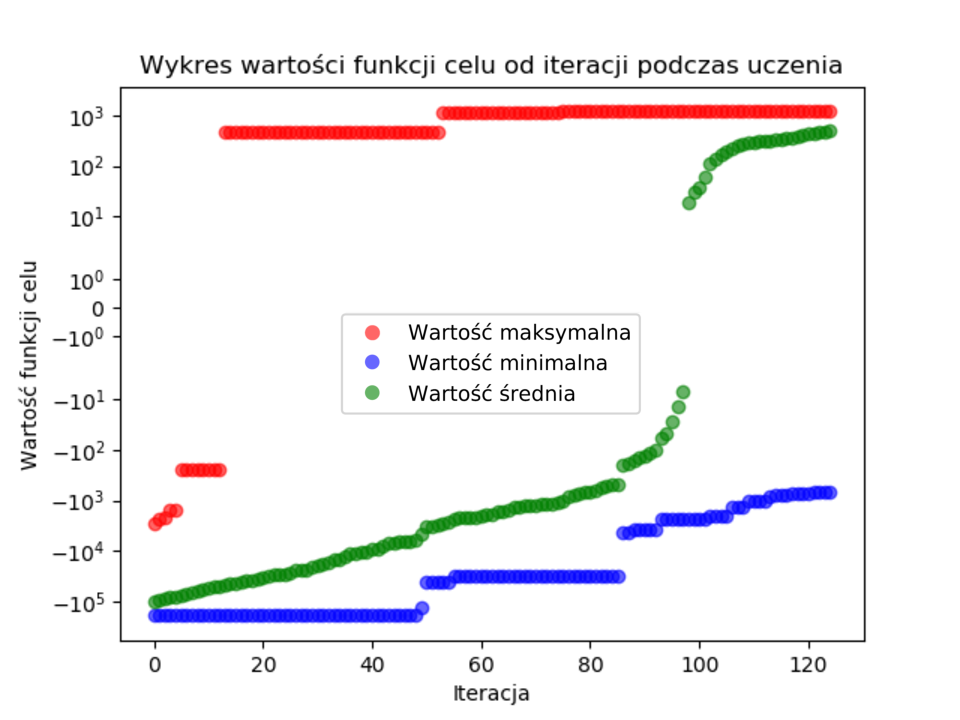
\includegraphics[width=0.7\textwidth]{plots/selection_05.pdf}
    \caption{Współczynnik wybieranych komórek = 5\%}
    \label{fig:selection_05}
\end{figure}

\begin{figure}[H]
    \centering
    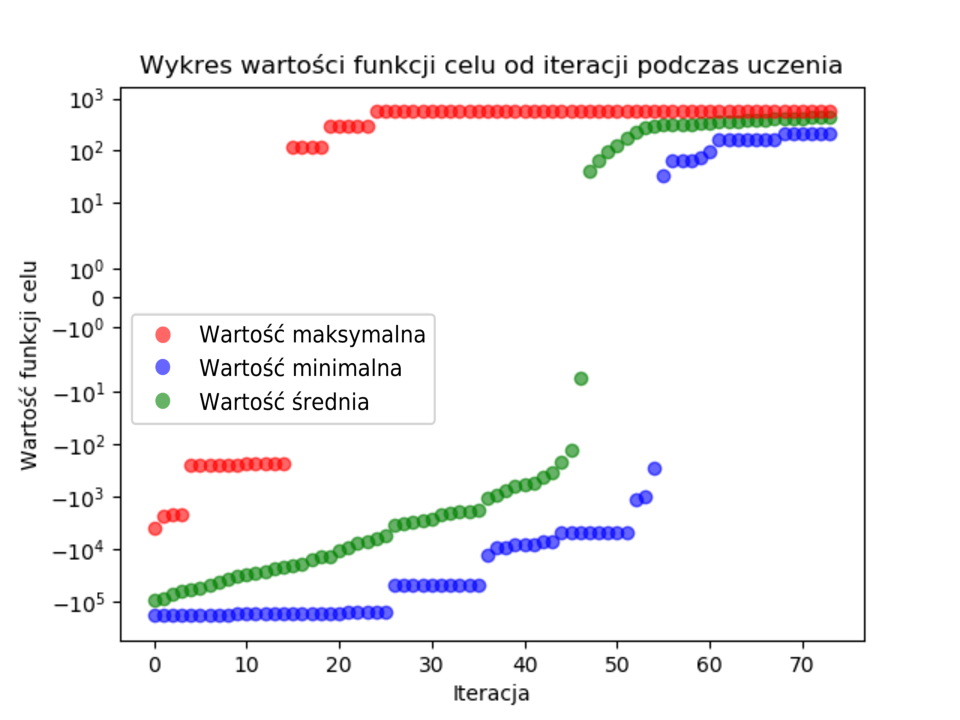
\includegraphics[width=0.7\textwidth]{plots/selection_10.pdf}
    \caption{Współczynnik wybieranych komórek = 10\%}
    \label{fig:selection_10}
\end{figure}

\begin{figure}[H]
    \centering
    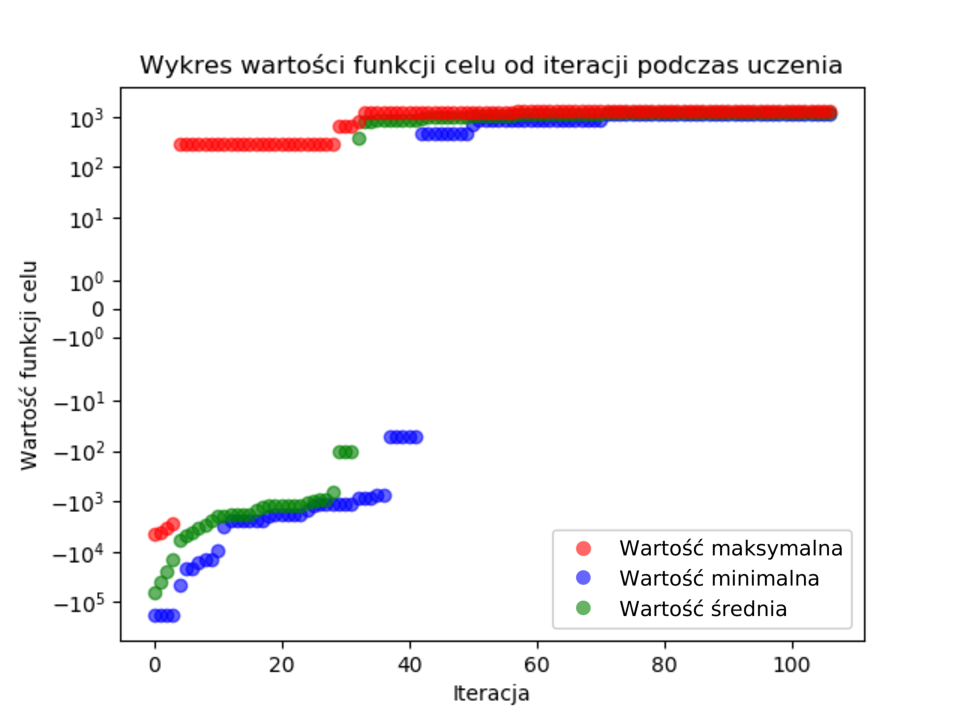
\includegraphics[width=0.7\textwidth]{plots/selection_40.pdf}
    \caption{Współczynnik wybieranych komórek = 40\%}
    \label{fig:selection_40}
\end{figure}

\begin{figure}[H]
    \centering
    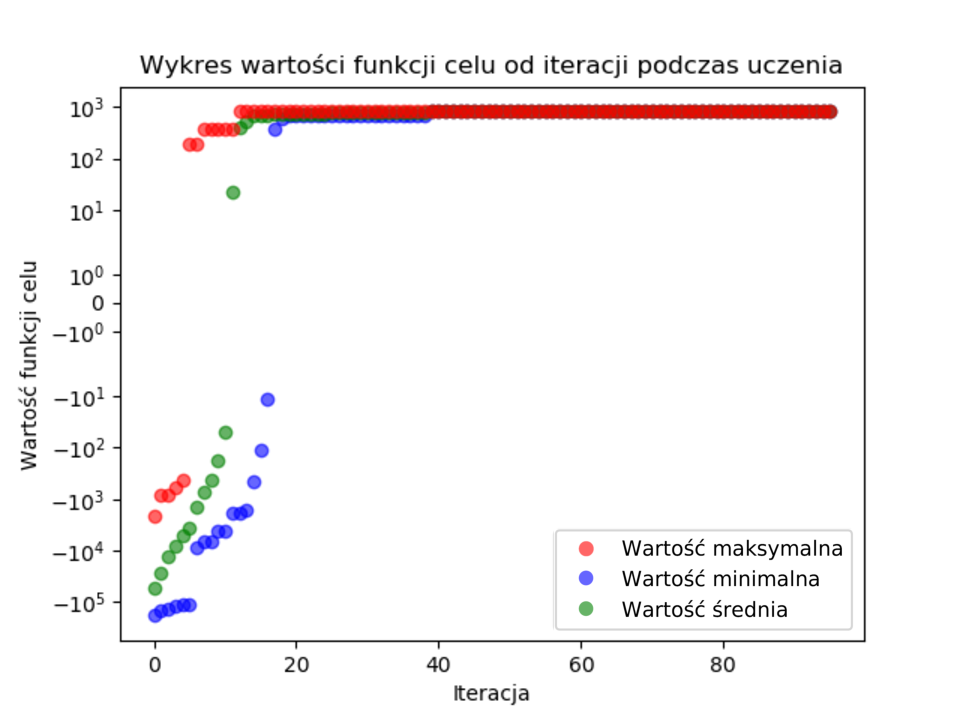
\includegraphics[width=0.7\textwidth]{plots/selection_50.pdf}
    \caption{Współczynnik wybieranych komórek = 50\%}
    \label{fig:selection_50}
\end{figure}


\subsection{Wnioski}
Wnioski wyciągnięte na podstawie analizy wykonanych testów z podziałem na poszczególne parametry.
\subsubsection{Wpływ zmian rozmiaru populacji}
Na podstawie przeprowadzonych testów można stwierdzić że rozmiar populacji mocno wpływa na wyniki symulacji. Wraz z wzrostem rozmiaru diametralnie poprawia się najlepszy osiągalny wynik. Im większa populacja tym więcej rozwiązań problemu porównujemy jednocześnie co, przy braku zmian pozostałych parametrów, naturalnie wiąże się z większą szansą na znalezienie lepszego rozwiązania. Dodatkowo można zauważyć że dla niewielkich populacji algorytm kończył się przed 200 (standardową) iteracją. Może być to powodowane tym że cała populacja "utyka" w lokalnym minimum i nie jest w stanie się z niego wydostać (ponieważ na podstawie innych testów wiemy że lepsze rozwiązania istnieją). Aby w przyszłości uniknąć takich sytuacji należało by lepiej dopasować współczynnik mutacji.
\subsubsection{Wpływ zmian liczby iteracji}
Na podstawie testów możemy stwierdzić iż liczba iteracji nie wpływa w znaczący sposób na rozwiązanie. Co było widoczne w wykonanych testach po pewnej liczbie iteracji wartość najlepszych rozwiązań "staje w miejscu". Wystarczy więc by ilość iteracji była na tyle duża by algorytm dotarł do miejsca zatrzymania się znaczącej poprawy. W związku z tym prawdopodobnie najlepiej było by uzależnić liczbę iteracji od innych parametrów. To że liczba iteracji nie wpływa bezpośrednio na najlepszą wartość uzyskaną przez algorytm można potwierdzić porównując test dla 40 i 100 iteracji. Przy 40 iteracjach rozwiązania "wpadły" w lepsze minimum lokalne i najlepszy wynik wyniósł około 1200, natomiast przy 100 iteracjach rozwiązania "wpadły" w gorsze minimum lokalne i po osiągnięciu pułapu 800 mimo dużej ilości iteracji nie były w stanie ulec znacznej poprawie.
\subsubsection{Wpływ zmian współczynnika klonowania}
Z testów wynika że współczynnik klonowania wpływa na jakość rozwiązań do pewnego stopnia. Naturalnie im większa liczba klonów, tym więcej mutacji, tym większa szansa że pojawi się rozwiązanie lepsze od obecnego. Jednak wraz z wzrostem parametru mocno zmienia się złożoność obliczeniowa. Wobec tego parametr należy dobrać optymalnie pod względem poprawy jakości rozwiązania i czasu wykonania algorytmu. Dodatkowo poprawa jakości wraz z wzrostem współczynnika wydaje się być coraz mniejsza co pozwala nam przypuszczać że odpowiednie optimum istnieje. Najlepsza wartość dla współczynnika o wartości 0.8 która jest mniejsza od najlepszej wartości dla współczynnika 0.6 wydaje się być dziełem przypadku a nie spadkiem jakości rozwiązania w związku z wzrostem współczynnika. Można dojść do takich wniosków na podstawie analizy działania całego algorytmu gdzie wzrost współczynnika nie ma możliwości osłabienia jakości rozwiązania najlepszego.
\subsubsection{Wpływ zmian watchdog-a}
Na podstawie testów można określić wpływ parametru watchdog na niewielki. Ma on wpływ na wynik algorytmu jedynie dla jego niewielkich wartości gdy algorytm w kilku krokach nie zdąży poprawić rozwiązań a watchdog jest na tyle mały że zakończy algorytm przed dojściem do maksimum wartości. Przy wielu testach nie udało się zaobserwować sytuacji w której najlepsze rozwiązanie nie zmieniałoby się przez ponad 40 iteracji a następnie uległo znacznej poprawie. Wydaje się więc że ustalenie wartości tego parametru na więcej niż 40, przy obecnym algorytmie, mija się z celem i jedynie wydłuża działanie algorytmu. 
\subsubsection{Wpływ zmian współczynnika wybranych komórek}
Zmiana parametru wydaje się nie mieć większego wpływu na jakość najlepszego rozwiązania.  Na podstawie analizy działania algorytmu można dojść do podobnych wniosków. Jako iż algorytm zastępuje rozwiązania tylko lepszymi rozwiązaniami, wybór dodatkowych gorszych rozwiązań do stworzenia klonów które i tak z dużym prawdopodobieństwem zostaną pominięte wydaje się być nieuzasadniony.

\section{Podsumowanie}

Algorytm immunologiczny selekcji klonalnej został wykorzystany w celu maksymalizacji funkcji celu utworzonego modelu fabryki. Przeprowadzone testy pokazują że w zależności od różnych ustawień parametrów, algorytm dąży do znalezienia najlepszego rezultatu. Uzyskane wartości funkcji celu są zadowalające. Należy mieć na uwadze, że ze względu na swój sposób działania, algorytm nie zawsze uzyska globalne optimum w każdym przypadku.

Dla ustalonych niedużych wartości parametrów liczby iteracji i rozmiaru populacji algorytm jest stosunkowo wydajny obliczeniowo, jednak niekiedy przekłada się to na gorszą jakość uzyskanych wyników. Z kolei dla większych wartości tych parametrów można wyraźnie odczuć, że zapotrzebowanie obliczeniowe jest większe, jednakże skutkuje to uzyskaniem lepszych rezultatów.

Reasumując, algorytm immunologiczny wykorzystujący zasadę selekcji klonalnej okazał się zdolny do zoptymalizowania postawionego problemu, niemniej jednak z powodzeniem może być stosowany do rozwiązywania różnych, innych problemów optymalizacyjnych.


\newpage
\printbibliography

\end{document}
